%-----------------------------------------------------------------------------
\section{Introdução}
%-----------------------------------------------------------------------------


%-----------------------------------------------------------------------------
\begin{frame}{Arduino}
\begin{figure}
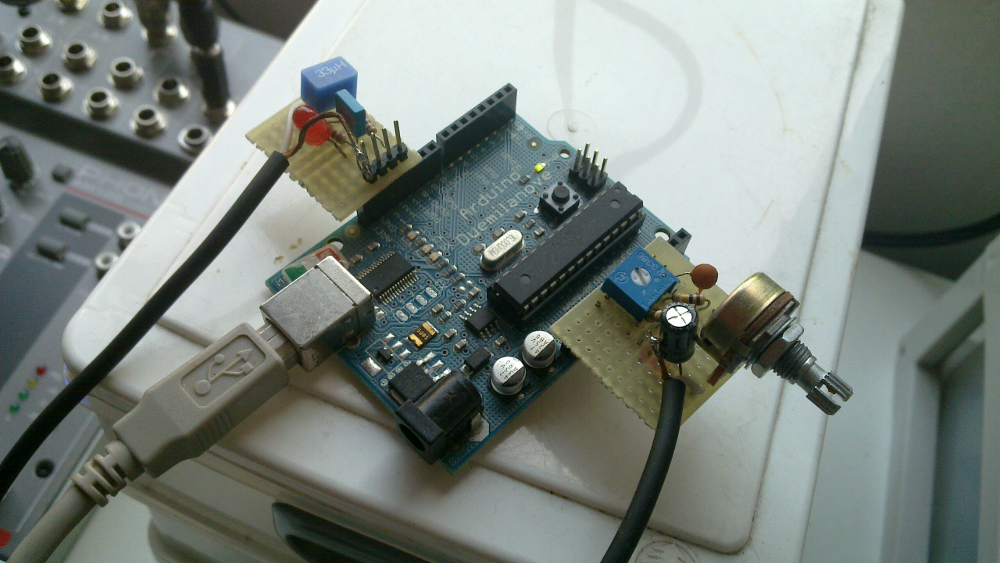
\includegraphics[width=\textwidth]{./img/arduino.png}
\end{figure}
\end{frame}
%-----------------------------------------------------------------------------


%-----------------------------------------------------------------------------
\begin{frame}{Arduino}{Características do projeto}
  \begin{itemize}
    \item Estrutura minimal para interface com um microcontrolador.
    \item Processing (MIT 2001) + Wiring (Ivrea 2003) $\rightarrow$ Arduino
    (Ivrea 2005).
    \item Geralmente usado como interface para controle.
    \item Baixo custo: 20-50 USD.
    \item Licenciamento livre:
    \begin{itemize}
      \item Projetos de hardware: CC BY-SA 2.5.
      \item Software: GPL (IDE) e LGPL (bibliotecas C/C++).
      \item Documentação: CC BY-SA 3.0.
    \end{itemize}
    \item Comunidade.
    \item Mobilidade.
    \item Expansibilidade.
  \end{itemize}
\end{frame}
%-----------------------------------------------------------------------------

%-----------------------------------------------------------------------------
\begin{frame}{Microcontroladores Atmel AVR (ATmega328P)}
\begin{itemize}
  \item CPU: unidade aritmética e registradores (16~MHz - 8 bits).
  \item Interrupções.
  \item Memórias: Flash (32~KB), SRAM (2~KB) e EEPROM (1~KB).
  \item Relógios de sistema (diversas fontes, pré-escalonadores).
  \item Gerenciamento de energia.
  \item Portas digitais de entrada e saída.
  \item Contadores (com PWM).
  \item Interface serial.
  \item Conversão analógico-digital.
  \item \emph{Boot-loader} e autoprogramação.
\end{itemize}
\end{frame}
%-----------------------------------------------------------------------------


%-----------------------------------------------------------------------------
\begin{frame}{Processamento Digital de Sinais de Áudio em tempo real}
Restrição de tempo máximo para o cálculo do resultado:
\begin{itemize}
    \item Período do bloco de processamento: $N$ amostras.
    \item Frequência de amostragem: $R$~Hz.
    \item Período do ciclo DSP: $T_{DSP}=\frac{N}{R}$~s.
\end{itemize}
\vspace{2em}
Perguntas:
\begin{itemize}
  \item Qual é o número máximo de operações que se pode realizar em tempo real?
  \item Quais detalhes de implementação fazem diferença?
  \item Qual é a qualidade do sinal de áudio resultante?
\end{itemize}
\end{frame}
%-----------------------------------------------------------------------------


